 %************************************************
\chapter{Cropped Training}\label{cropped-training}
%**************************************

\begin{startbox}{Cropped training means training on many temporal windows within one input example}  
\item Greatly increases the number of training examples
\item Can be made computationally efficient by avoiding redundant computations
\end{startbox}


    In this chapter, we describe a training strategy called ``cropped
training'' which addresses the problem of the relatively low number of
training examples in typical EEG datasets. The goal of this strategy is
to improve the performance of deep networks by training them on many
sliding temporal windows within the data. This approach had been
similarly used as spatial cropping in computer vision, where networks
are trained on multiple cropped versions of images. We first describe
the concept of regular, non-cropped training and then introduce cropped
training on a conceptual level. Finally, we discuss how to implement
this approach efficiently. Our aim is to demonstrate the effectiveness
and computational efficiency of cropped training as a regularization
technique for deep networks on EEG data.

Cropped training for EEG decoding was developed by me in the context of
this thesis. Some text and figures are adapted from from
\cite{schirrmeisterdeephbm2017}.


\section{Non-Cropped/Trialwise
Training}\label{non-croppedtrialwise-training}



\begin{figure}[bth]
    \myfloatalign
    \subfloat[\textbf{Trialwise training.} An entire single trial is fed
through the network and the network's prediction is compared to the
trial target to train the network.]
    {\label{trialwise-figure}
    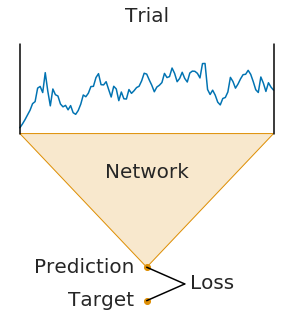
\includegraphics[width=.4\linewidth]{images/trialwise_explanation.png}} \quad
    \subfloat[\textbf{Cropped training.} A compute window contains many
temporal windows (crops) inside that are used as individual examples to
train the network.]
    {\label{cropped-figure}%
        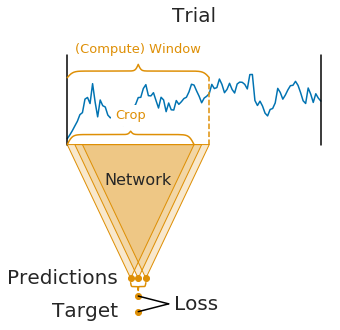
\includegraphics[width=.464\linewidth]{images/cropped_explanation.png}} 
    \caption[Trialwise and cropped training]{\textbf{Trialwise and cropped training.}}\label{cropped-and-trialwise-figure}
\end{figure}


In the trialwise training of neural networks on EEG data, each example
consists of the EEG signals from a single trial and its corresponding
label (see \Cref{trialwise-figure}). This might for example be a 4-second-trial where a subject moved
the left hand, with the 4-second-signal as the input and the left hand
as a label. Due to the typically small size of EEG datasets, networks
trained in this way may only be trained on a few hundred to a few
thousand examples per subject. This is significantly fewer examples than
those used to train networks in computer vision, where tens of thousands
or even millions of images are commonly used.


\section{Cropped Training}\label{cropped-training-section}

Cropped training increases the number of training examples by training
on many crops, i.e., temporal windows, within the trial (see \Cref{cropped-figure}). For example, in
a 4-second trial, all possible 2-second windows within the trial could
be used as ``independent'' examples. This approach drastically increases
the number of training examples, although many of the examples are
highly overlapping. This can be seen as an extreme version of using
random crops of images which is a method used to train deep networks in
computer vision. A naive implementation of cropped training would
greatly increase the computational cost per epoch due to the highly
increased number of examples. Thankfully, the high overlap between
neighbouring crops can be exploited for a more efficient implementation.



\section{Computationally Faster Cropped
Training}\label{computationally-faster-cropped-training}


\begin{figure}[ht]
    \myfloatalign
    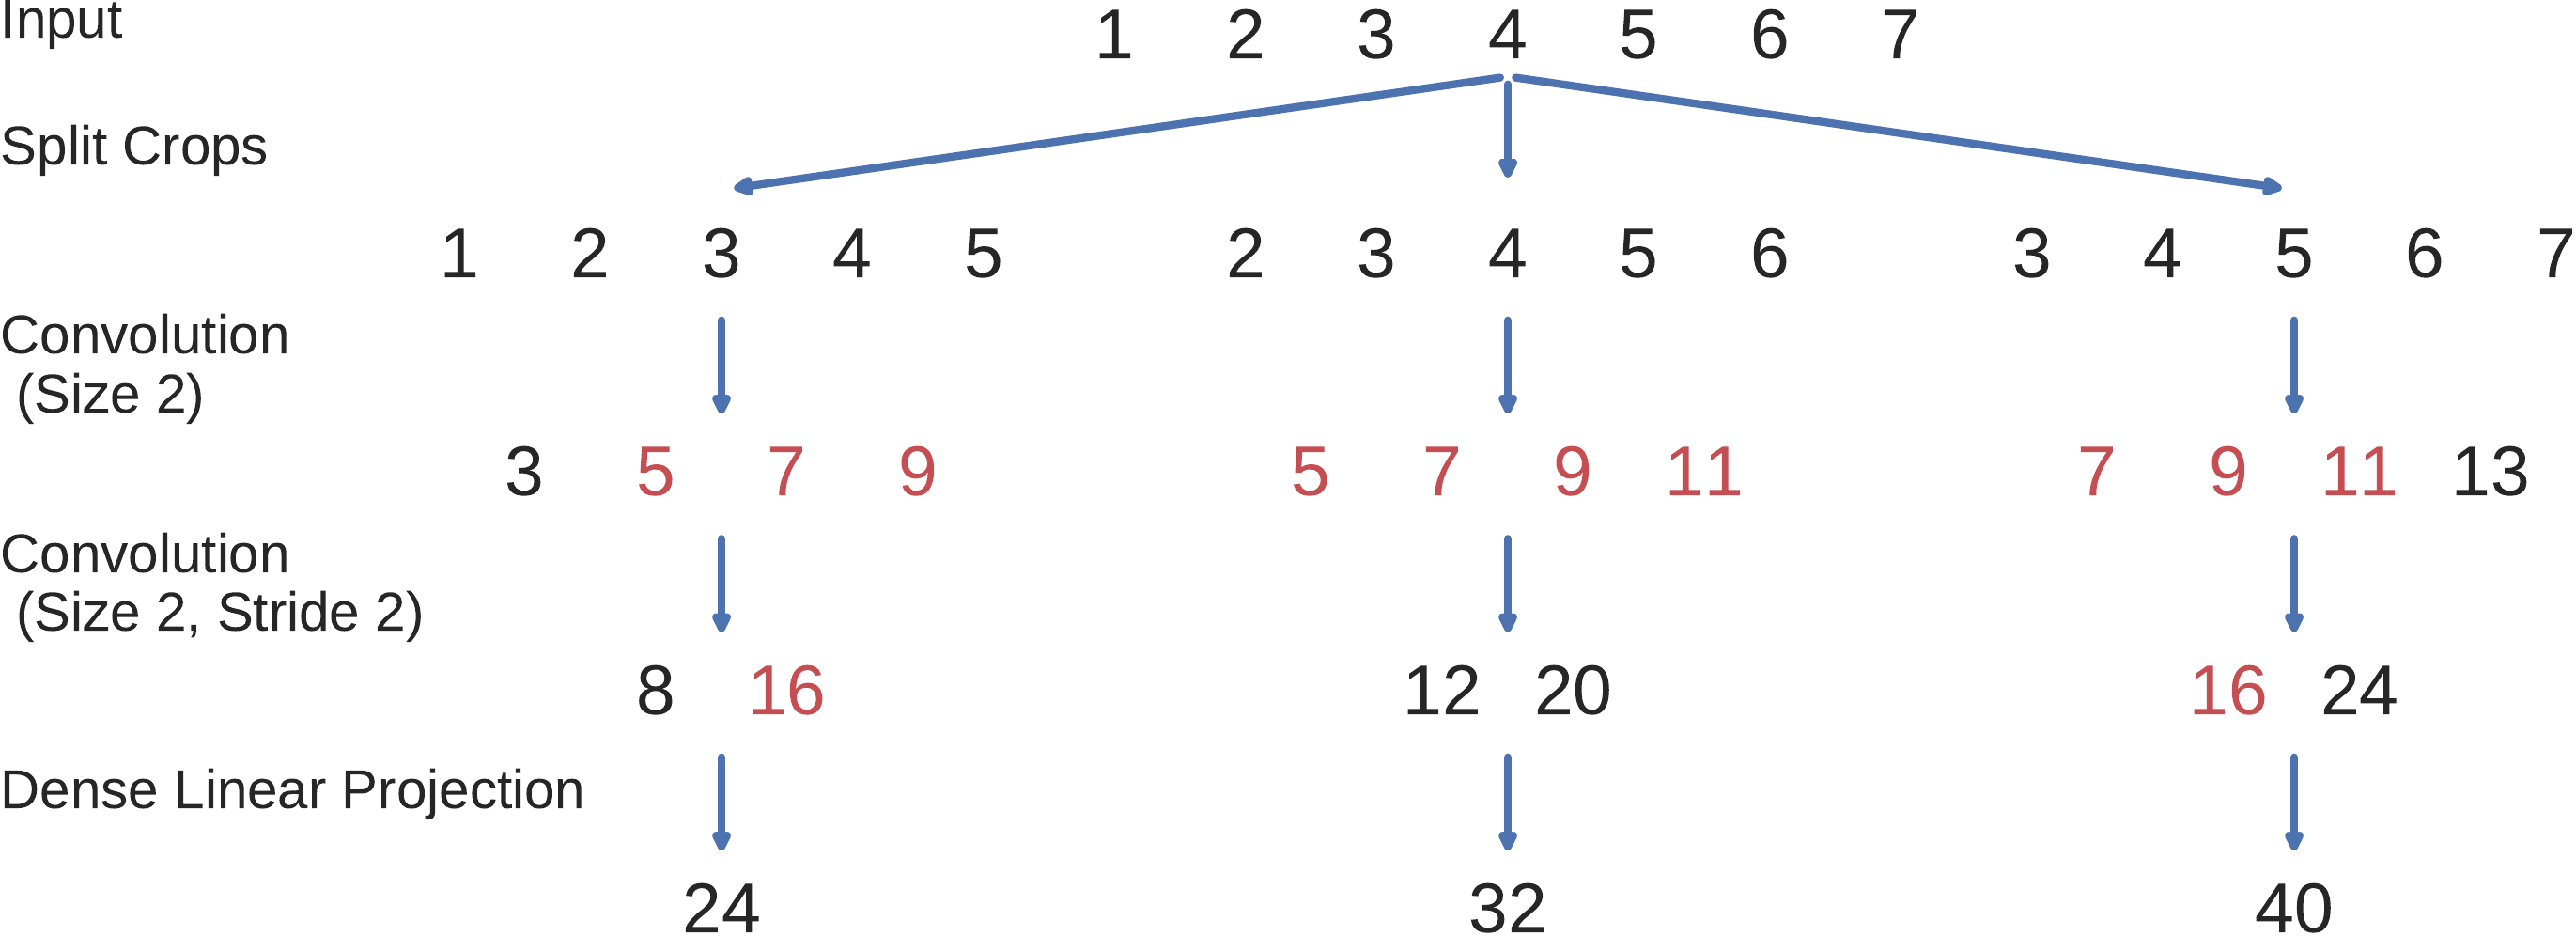
\includegraphics[width=1\linewidth]{images/Multiple_Prediction_Matplotlib_Graphics.ipynb.2.png}
    \caption[Naive cropped training toy example]{
\textbf{Naive cropped training toy example.} Each possible length-5 crop
is taken from the original length-7 trial and independently processed by
the Conv-Conv-Linear projection network. All filter values of the
network are assumed to be ones. Each crop is processed independently.
The values in red are identical and unnecessarily computed independently
for each crop. Figure from \cite{schirrmeisterdeephbm2017}.
}
\label{cropped-naive-computation-figure}
\end{figure}


\begin{figure}[ht]
    \myfloatalign
    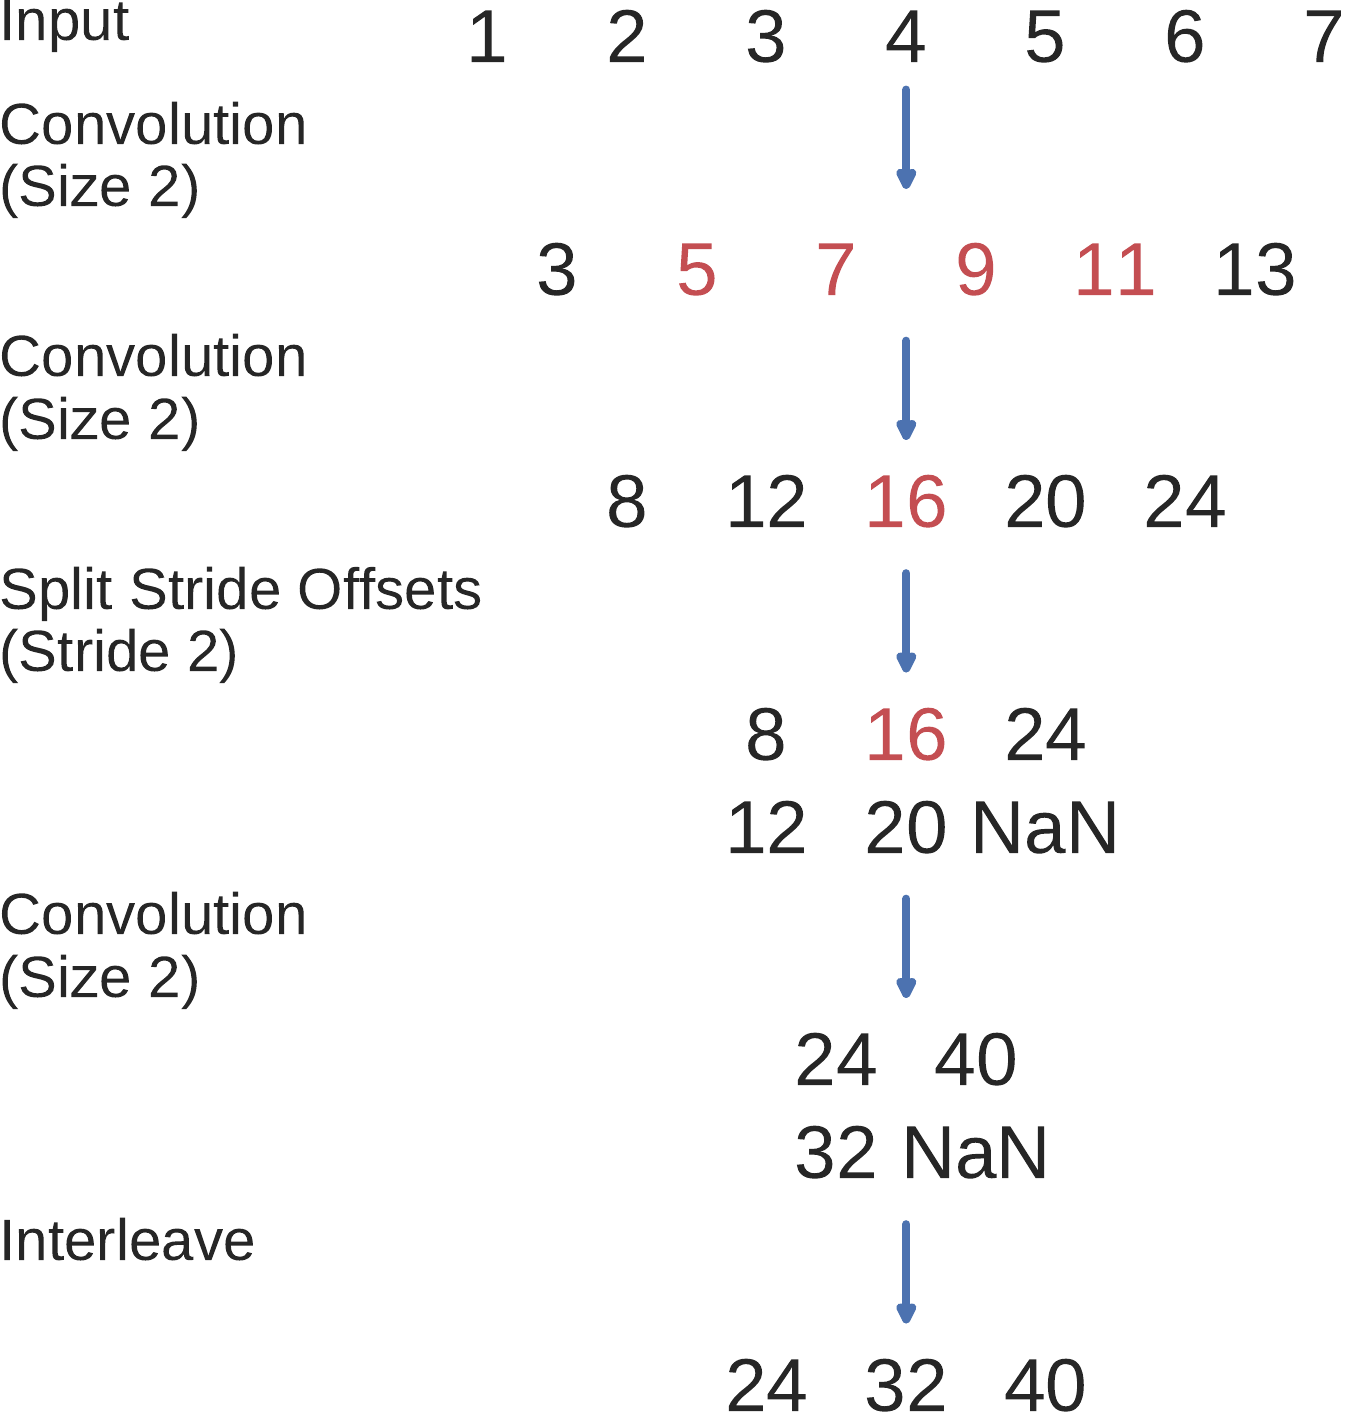
\includegraphics[width=0.5\linewidth]{images/Multiple_Prediction_Matplotlib_Graphics.ipynb.3.png}
    \caption[Efficient cropped training]{
    \textbf{Efficient cropped training.} Each possible length-5 crop is
    taken from the original length-7 trial and processed simultaneously by
    the Conv-Conv-Linear projection network, whilce still yielding the same
    results as if processed independently
    (\Cref{cropped-efficient-computation-figure}). All filter
    values of the network are assumed to be ones. Figure from
    \cite{schirrmeisterdeephbm2017}.
}
\label{cropped-efficient-computation-figure}
\end{figure}


    Cropped training can be implemented with substantially less computations
by exploiting that highly overlapping crops result in highly overlapping
intermediate network activations. By passing a group of neighbouring
crops together to the network, we can reuse intermediate computations.
See \Cref{cropped-naive-computation-figure} and
\Cref{cropped-efficient-computation-figure} for a concrete
example of this speedup method. This idea had been used in the same way
for dense predictions on images, e.g., for segmentation
\citep{giusti_fast_2013,nasse_face_2009,sermanet_overfeat:_2013,shelhamer_fully_2016}.

    Efficient cropped training then results in the exact same predictions
and training as if the neighbouring crops were passed separately through
the network. This is only true for networks that either use left-padding
or no padding at all to the input and the intermediate activations. In
the deep and shallow network described here, we do not use any padding.
In the residual network, we use padding, hence the training is not
exactly identical to passing neighbouring crops separately, but we still
found it to improve over trial-wise training.

    The more efficient way to do cropped training introduces a new
hyperparameter, the number of neighbouring crops that are decoded
together. The larger this hyperparameter, the more computations are
saved and the more speedup one gets (see
\citet{giusti_fast_2013} for a more detailed speedup analysis
on images). Larger numbers of neighbouring crops to simultaneously train
on require more memory and may also affect the training dynamics due to
more neighbouring crops being in the same mini-batch. However, we did
not find negative effects on the training dynamics from larger number of
simultaneously decoded neighbouring crops, consistent with prior work in
computer vision \citep{shelhamer_fully_2016}.

\begin{openbox}
\item For which datasets and architectures does cropped training help or hurt? 
\end{openbox}
